% Created by tikzDevice version 0.12.3 on 2019-12-11 20:53:24
% !TEX encoding = UTF-8 Unicode
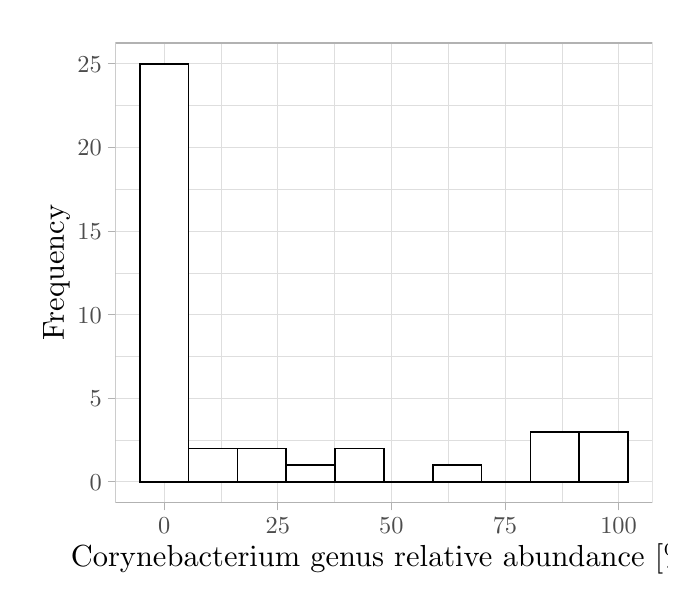
\begin{tikzpicture}[x=1pt,y=1pt]
\definecolor{fillColor}{RGB}{255,255,255}
\path[use as bounding box,fill=fillColor,fill opacity=0.00] (0,0) rectangle (231.26,202.36);
\begin{scope}
\path[clip] (  0.00,  0.00) rectangle (231.26,202.36);
\definecolor{drawColor}{RGB}{255,255,255}
\definecolor{fillColor}{RGB}{255,255,255}

\path[draw=drawColor,line width= 0.6pt,line join=round,line cap=round,fill=fillColor] (  0.00,  0.00) rectangle (231.26,202.36);
\end{scope}
\begin{scope}
\path[clip] ( 31.71, 30.69) rectangle (225.76,196.86);
\definecolor{fillColor}{RGB}{255,255,255}

\path[fill=fillColor] ( 31.71, 30.69) rectangle (225.76,196.86);
\definecolor{drawColor}{gray}{0.87}

\path[draw=drawColor,line width= 0.1pt,line join=round] ( 31.71, 53.35) --
	(225.76, 53.35);

\path[draw=drawColor,line width= 0.1pt,line join=round] ( 31.71, 83.56) --
	(225.76, 83.56);

\path[draw=drawColor,line width= 0.1pt,line join=round] ( 31.71,113.77) --
	(225.76,113.77);

\path[draw=drawColor,line width= 0.1pt,line join=round] ( 31.71,143.98) --
	(225.76,143.98);

\path[draw=drawColor,line width= 0.1pt,line join=round] ( 31.71,174.20) --
	(225.76,174.20);

\path[draw=drawColor,line width= 0.1pt,line join=round] ( 69.87, 30.69) --
	( 69.87,196.86);

\path[draw=drawColor,line width= 0.1pt,line join=round] (110.91, 30.69) --
	(110.91,196.86);

\path[draw=drawColor,line width= 0.1pt,line join=round] (151.94, 30.69) --
	(151.94,196.86);

\path[draw=drawColor,line width= 0.1pt,line join=round] (192.98, 30.69) --
	(192.98,196.86);

\path[draw=drawColor,line width= 0.3pt,line join=round] ( 31.71, 38.24) --
	(225.76, 38.24);

\path[draw=drawColor,line width= 0.3pt,line join=round] ( 31.71, 68.45) --
	(225.76, 68.45);

\path[draw=drawColor,line width= 0.3pt,line join=round] ( 31.71, 98.66) --
	(225.76, 98.66);

\path[draw=drawColor,line width= 0.3pt,line join=round] ( 31.71,128.88) --
	(225.76,128.88);

\path[draw=drawColor,line width= 0.3pt,line join=round] ( 31.71,159.09) --
	(225.76,159.09);

\path[draw=drawColor,line width= 0.3pt,line join=round] ( 31.71,189.30) --
	(225.76,189.30);

\path[draw=drawColor,line width= 0.3pt,line join=round] ( 49.35, 30.69) --
	( 49.35,196.86);

\path[draw=drawColor,line width= 0.3pt,line join=round] ( 90.39, 30.69) --
	( 90.39,196.86);

\path[draw=drawColor,line width= 0.3pt,line join=round] (131.43, 30.69) --
	(131.43,196.86);

\path[draw=drawColor,line width= 0.3pt,line join=round] (172.46, 30.69) --
	(172.46,196.86);

\path[draw=drawColor,line width= 0.3pt,line join=round] (213.50, 30.69) --
	(213.50,196.86);
\definecolor{drawColor}{RGB}{0,0,0}

\path[draw=drawColor,line width= 0.6pt,line cap=rect,fill=fillColor] ( 40.53, 38.24) rectangle ( 58.17,189.30);

\path[draw=drawColor,line width= 0.6pt,line cap=rect,fill=fillColor] ( 58.17, 38.24) rectangle ( 75.81, 50.32);

\path[draw=drawColor,line width= 0.6pt,line cap=rect,fill=fillColor] ( 75.81, 38.24) rectangle ( 93.46, 50.32);

\path[draw=drawColor,line width= 0.6pt,line cap=rect,fill=fillColor] ( 93.46, 38.24) rectangle (111.10, 44.28);

\path[draw=drawColor,line width= 0.6pt,line cap=rect,fill=fillColor] (111.10, 38.24) rectangle (128.74, 50.32);

\path[draw=drawColor,line width= 0.6pt,line cap=rect,fill=fillColor] (128.74, 38.24) rectangle (146.38, 38.24);

\path[draw=drawColor,line width= 0.6pt,line cap=rect,fill=fillColor] (146.38, 38.24) rectangle (164.02, 44.28);

\path[draw=drawColor,line width= 0.6pt,line cap=rect,fill=fillColor] (164.02, 38.24) rectangle (181.66, 38.24);

\path[draw=drawColor,line width= 0.6pt,line cap=rect,fill=fillColor] (181.66, 38.24) rectangle (199.30, 56.37);

\path[draw=drawColor,line width= 0.6pt,line cap=rect,fill=fillColor] (199.30, 38.24) rectangle (216.94, 56.37);
\definecolor{drawColor}{gray}{0.70}

\path[draw=drawColor,line width= 0.6pt,line join=round,line cap=round] ( 31.71, 30.69) rectangle (225.76,196.86);
\end{scope}
\begin{scope}
\path[clip] (  0.00,  0.00) rectangle (231.26,202.36);
\definecolor{drawColor}{gray}{0.30}

\node[text=drawColor,anchor=base east,inner sep=0pt, outer sep=0pt, scale=  0.88] at ( 26.76, 35.21) {0};

\node[text=drawColor,anchor=base east,inner sep=0pt, outer sep=0pt, scale=  0.88] at ( 26.76, 65.42) {5};

\node[text=drawColor,anchor=base east,inner sep=0pt, outer sep=0pt, scale=  0.88] at ( 26.76, 95.63) {10};

\node[text=drawColor,anchor=base east,inner sep=0pt, outer sep=0pt, scale=  0.88] at ( 26.76,125.85) {15};

\node[text=drawColor,anchor=base east,inner sep=0pt, outer sep=0pt, scale=  0.88] at ( 26.76,156.06) {20};

\node[text=drawColor,anchor=base east,inner sep=0pt, outer sep=0pt, scale=  0.88] at ( 26.76,186.27) {25};
\end{scope}
\begin{scope}
\path[clip] (  0.00,  0.00) rectangle (231.26,202.36);
\definecolor{drawColor}{gray}{0.70}

\path[draw=drawColor,line width= 0.3pt,line join=round] ( 28.96, 38.24) --
	( 31.71, 38.24);

\path[draw=drawColor,line width= 0.3pt,line join=round] ( 28.96, 68.45) --
	( 31.71, 68.45);

\path[draw=drawColor,line width= 0.3pt,line join=round] ( 28.96, 98.66) --
	( 31.71, 98.66);

\path[draw=drawColor,line width= 0.3pt,line join=round] ( 28.96,128.88) --
	( 31.71,128.88);

\path[draw=drawColor,line width= 0.3pt,line join=round] ( 28.96,159.09) --
	( 31.71,159.09);

\path[draw=drawColor,line width= 0.3pt,line join=round] ( 28.96,189.30) --
	( 31.71,189.30);
\end{scope}
\begin{scope}
\path[clip] (  0.00,  0.00) rectangle (231.26,202.36);
\definecolor{drawColor}{gray}{0.70}

\path[draw=drawColor,line width= 0.3pt,line join=round] ( 49.35, 27.94) --
	( 49.35, 30.69);

\path[draw=drawColor,line width= 0.3pt,line join=round] ( 90.39, 27.94) --
	( 90.39, 30.69);

\path[draw=drawColor,line width= 0.3pt,line join=round] (131.43, 27.94) --
	(131.43, 30.69);

\path[draw=drawColor,line width= 0.3pt,line join=round] (172.46, 27.94) --
	(172.46, 30.69);

\path[draw=drawColor,line width= 0.3pt,line join=round] (213.50, 27.94) --
	(213.50, 30.69);
\end{scope}
\begin{scope}
\path[clip] (  0.00,  0.00) rectangle (231.26,202.36);
\definecolor{drawColor}{gray}{0.30}

\node[text=drawColor,anchor=base,inner sep=0pt, outer sep=0pt, scale=  0.88] at ( 49.35, 19.68) {0};

\node[text=drawColor,anchor=base,inner sep=0pt, outer sep=0pt, scale=  0.88] at ( 90.39, 19.68) {25};

\node[text=drawColor,anchor=base,inner sep=0pt, outer sep=0pt, scale=  0.88] at (131.43, 19.68) {50};

\node[text=drawColor,anchor=base,inner sep=0pt, outer sep=0pt, scale=  0.88] at (172.46, 19.68) {75};

\node[text=drawColor,anchor=base,inner sep=0pt, outer sep=0pt, scale=  0.88] at (213.50, 19.68) {100};
\end{scope}
\begin{scope}
\path[clip] (  0.00,  0.00) rectangle (231.26,202.36);
\definecolor{drawColor}{RGB}{0,0,0}

\node[text=drawColor,anchor=base,inner sep=0pt, outer sep=0pt, scale=  1.10] at (128.74,  7.64) {Corynebacterium genus relative abundance [\%]};
\end{scope}
\begin{scope}
\path[clip] (  0.00,  0.00) rectangle (231.26,202.36);
\definecolor{drawColor}{RGB}{0,0,0}

\node[text=drawColor,rotate= 90.00,anchor=base,inner sep=0pt, outer sep=0pt, scale=  1.10] at ( 13.08,113.77) {Frequency};
\end{scope}
\end{tikzpicture}
